% !TEX program = xelatex
\documentclass[12pt]{article}
\usepackage{fontspec}
\usepackage{tabularx}
\usepackage{xeCJK}
\usepackage{chemformula}
\usepackage{booktabs, longtable}
\usepackage{multirow}
\setmainfont[Path=fonts/, BoldFont=*-Bold, UprightFont=*-regular, ItalicFont=*-It]{MinionPro}
\setCJKmainfont[Path=fonts/]{HanaMinA.ttf}
\setCJKmonofont[Path=fonts/]{HanaMinA.ttf}
\usepackage[vmargin=1in,hmargin=0.5in]{geometry}
\usepackage{fancyhdr}
\pagestyle{fancy}
\fancyhf{}
\rhead{ISO/IEC JTC1/SC2/WG2/IRG N2578JunliangFeedback}
\lhead{Universal Multiple-Octet Coded Character Set}
\cfoot{\thepage}
\usepackage{caption}
\usepackage[pdfusetitle]{hyperref}
\usepackage{graphicx}
\graphicspath{{images}}
\usepackage{cite}

\makeatletter
\newcommand\HUGE{\@setfontsize\Huge{40}{50}}
\makeatother    

\newcommand{\glyphC}[0]{{\CJKfontspec[Path=fonts/]{u2ff0-u2ff3-u4e00-u5ddb-u5382-u5145-var-001.ttf}〓}}
\newcommand{\glyphQ}[0]{{\CJKfontspec[Path=fonts/]{u2ff0-u2ff3-u4e00-u5ddb-u5382-u6b20-var-001.ttf}〓}}
\newcommand{\glyphS}[0]{{\CJKfontspec[Path=fonts/]{u2ff0-u2ff3-u4e00-u5ddb-u5382-u5c11-var-001}〓}}
\newcommand{\glyphW}[0]{{\CJKfontspec[Path=fonts/]{u2ff4-u56d7-u2ff3-u4e00-u5ddb-u5382.ttf}〓}}
\newcommand{\glyphCOne}[0]{{\CJKfontspec[Path=fonts/]{irg2021-00016.ttf}〓}}
\newcommand{\glyphCTwo}[0]{{\CJKfontspec[Path=fonts/]{irg2021-00017.ttf}〓}}
\newcommand{\glyphQTwo}[0]{{\CJKfontspec[Path=fonts/]{irg2021-01900.ttf}〓}}
\newcommand{\glyphSTwo}[0]{{\CJKfontspec[Path=fonts/]{irg2021-00014.ttf}〓}}
\newcommand{\glyphCThree}[0]{{\CJKfontspec[Path=fonts/]{u2ff0-u2ff3-u4e00-u5ddb-u2ff8-u5382-u4e09-u5145-var-001.ttf}〓}}
\newcommand{\glyphQThree}[0]{{\CJKfontspec[Path=fonts/]{u2ff0-u2ff3-u4e00-u5ddb-u2ff8-u5382-u4e09-u6b20-var-001.ttf}〓}}
\newcommand{\glyphSThree}[0]{{\CJKfontspec[Path=fonts/]{u2ff0-u2ff3-u4e00-u5ddb-u2ff8-u5382-u4e09-u5c11-var-001.ttf}〓}}
\newcommand{\glyphCFour}[0]{{\CJKfontspec[Path=fonts/]{u2ff0-u2ff3-u4e00-u5ddb-u2ff8-u5382-u56db-u5145-var-001.ttf}〓}}
\newcommand{\glyphQFour}[0]{{\CJKfontspec[Path=fonts/]{u2ff0-u2ff3-u4e00-u5ddb-u2ff8-u5382-u56db-u6b20.ttf}〓}}
\newcommand{\glyphCFive}[0]{{\CJKfontspec[Path=fonts/]{u2ff0-u2ff3-u4e00-u5ddb-u2ff8-u5382-u4e94-u5145-var-001.ttf}〓}}
\newcommand{\glyphWFive}[0]{{\CJKfontspec[Path=fonts/]{u2ff4-u56d7-u2ff3-u4e00-u5ddb-u2ff8-u5382-u4e94.ttf}〓}}
\newcommand{\glyphWSix}[0]{{\CJKfontspec[Path=fonts/]{irg2021-00777.ttf}〓}}
\newcommand{\glyphCFifteen}[0]{{\CJKfontspec[Path=fonts/]{jlhwung_u2ff0-u2ff3-u4e00-u5ddb-u2ff8-u5382-u2ff1-u5341-u4e94-u5145.ttf}〓}}
\newcommand{\glyphCSixteen}[0]{{\CJKfontspec[Path=fonts/]{jlhwung_u2ff0-u2ff3-u4e00-u5ddb-u2ff8-u5382-u2ff1-u5341-u516d-u5145.ttf}〓}}
\newcommand{\glyphCNineteen}[0]{{\CJKfontspec[Path=fonts/]{u2ff0-u2ff3-u4e00-u5ddb-u2ff8-u5382-u2ff1-u5341-u4e5d-u5145.ttf}〓}}
\newcommand{\glyphCTwentyOne}[0]{{\CJKfontspec[Path=fonts/]{u2ff0-u2ff3-u4e00-u5ddb-u2ff8-u5382-u2ff1-u5eff-u4e00-u5145.ttf}〓}}
\newcommand{\glyphCSixty}[0]{{\CJKfontspec[Path=fonts/]{u2ff0-u2ff3-u4e00-u5ddb-u2ff8-u5382-u2ff1-u516d-u5341-u5145.ttf}〓}}

\setlength{\headheight}{15pt}

\begin{document}
\title{Feedback on IRGN2578 ``Comments on encoding early Chinese organic chemical character in WS2021 and other complex ideographs"}
\author{Huáng Jùnliàng (黃俊亮)}

\makeatletter
\begin{tabularx}{.9\textwidth}{l X}
Doc Type: & Working Group Document \\

Title: & \@title\footnotemark \\

Source: & \@author \\

Status: & Individual contribution \\

Action required: & To be considered by the IRG and UTC \\

Date: & \today \\
\end{tabularx}
\makeatother
\footnotetext{Sources of this document are available online: \url{https://github.com/JLHwung/IRGN2578Feedback}.}

\vspace{\baselineskip}

In IRGN2578, Eiso Chan listed four base characters of the first type of early organic chemical characters: \glyphC, \glyphQ, \glyphS and \glyphW. Additionally, Chan noted the importance of checking historical usage of numerals greater than 10 when combined with these base characters. To recap, the combined characters are instances of the hydrocarbon nomenclature first proposed by 梁國常 in his work 有機化學命名芻議\cite{有機化學命名芻議}.

Table \ref{table:unencoded} contains a list of unencoded hydrocarbon characters based on evidence from Liang's work.

\begin{longtable}[c]{c c c}
\caption[]{Unencoded hydrocarbon characters in Liang's work not submitted for WS2021}\label{table:unencoded}\\
\toprule
Character & Page & Evidence \\
\midrule[\heavyrulewidth]
\endfirsthead
\toprule
Character & Page & Evidence \\
\midrule[\heavyrulewidth]
\endhead

{\HUGE \glyphC} & 73 & 
\includegraphics[height=30pt]{c-evidence.png} \\\midrule
{\HUGE \glyphQ} & 73 & 
\includegraphics[height=35pt]{q-evidence.png} \\\midrule
{\HUGE \glyphS} & 73 & 
\includegraphics[height=32pt]{s-evidence.png} \\\midrule
{\HUGE \glyphW} & 73 & 
\includegraphics[height=27pt]{w-evidence.png} \\\midrule
{\HUGE \glyphCThree} & 73 & 
\includegraphics[height=50pt]{c3-evidence.png} \\\midrule
{\HUGE \glyphQThree} & 78 & 
\includegraphics[height=39pt]{q3-evidence.png} \\\midrule
{\HUGE \glyphSThree} & 78 & 
\includegraphics[height=40pt]{s3-evidence.png} \\\midrule
{\HUGE \glyphCFour} & 73 & 
\includegraphics[height=40pt]{c4-evidence.png} \\\midrule 
{\HUGE \glyphQFour} & 78 & 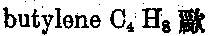
\includegraphics[height=40pt]{q4-evidence.png} \\\midrule
{\HUGE \glyphCFive} & 81 & 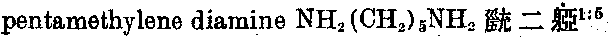
\includegraphics[height=26pt]{c5-evidence.png} \\\midrule
\multirow{2}{*}{\HUGE \glyphWFive} & 73 & 
\includegraphics[height=40pt]{w5-evidence-1.png} \\
& 88 & 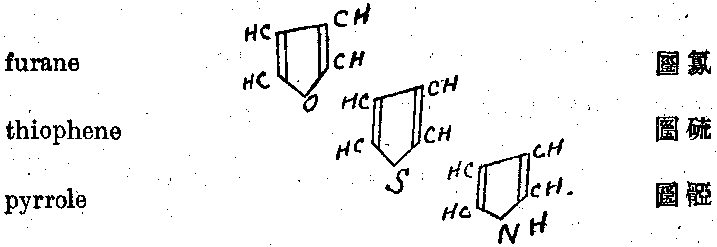
\includegraphics[height=145pt]{w5-evidence-2.png} \\\midrule
\multirow{2}{*}{\HUGE \glyphCFifteen}\footnotemark
& 81 & 
\includegraphics[height=21pt]{c15-evidence-2.png} \\
& 81 & 
\includegraphics[height=33pt]{c15-evidence-1.png} \\\midrule
{\HUGE \glyphCNineteen} & 80 & 
\includegraphics[height=36pt]{c19-evidence.png} \\\midrule
{\HUGE \glyphCTwentyOne} & 78 & 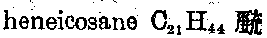
\includegraphics[height=46pt]{c21-evidence.png} \\\midrule
{\HUGE \glyphCSixty} & 78 & 
\includegraphics[height=46pt]{c60-evidence.png} \\
\bottomrule
\end{longtable}
\footnotetext{To clarify, in the presented evidences, it would be more accurate to use \glyphCSixteen instead of \glyphCFifteen, as both tripalmitin and monopalmitin contain hexadecanoate (\ch{C16H31O2-}) rather than pentadecanoate (\ch{C15H29O2-}).} 

If we are to encode \glyphCOne (00016), \glyphCTwo (00017), \glyphQTwo (01900), \glyphSTwo (00014) and \glyphWSix (00777) one by one, then we should also encode the other 15 characters above in order to digitize Liang's work. In total, we need to encode 20 characters, which is already more than the length of a minimal Unicode block (16 characters), should they be encoded as IDJ sequences proposed in IRGN2578.

Additionally, it's important to note that hydrocarbons can have an arbitrary number of carbon atoms, making such characters an open set. It's possible that Liang's nomenclature was adopted in other historical documents, which may contain additional hydrocarbon characters that we're currently unaware of. In other words, we may have to encode more than 20 hydrocarbon characters in the future.

To summarize, encoding hydrocarbon characters as IDJ sequences can help us save codepoint space and address the open set nature of Liang's nomenclature. As presented in IRGN2578, the IDJ approach potentially solve other encoding issues, too. In light of this I recommend that we carefully consider Chan's approach and inform our encoding strategy.

\section*{Acknowledgements}
``Hulenkius" helps me polish the font.

\bibliography{main}
\bibliographystyle{IEEEtran}

\vfill
(End of Document)

\end{document}